\documentclass[simplex.tex]{subfiles}
% DO NOT INCLUDE PREAMBLES/PACKAGES HERE!!
% packages are inherited from preamble.tex; you can compile this on its own
\providecommand{\sct}[1]{{\normalfont\textsc{#1}}}
\newcommand{\Hhg}{\sct{Hhg}}
\newcommand{\Mgc}{\sct{Mgc}}
\begin{document}
 
\subsection{Multiscale Generalized Correlation (MGC)}

We developed the Multiscale Generalized Correlation method to better detect associations between two datasets $X$ and $Y$. We demonstrate that Oracle MGC is a consistent test statistic (power converge to 1 as sample size increases) under standard regularity conditions, is equivalently to the global correlation under linear dependency (i.e., each observation $X_i$ is a linear transformation of $Y_i$), and can be strictly better than the global correlation under common nonlinear dependencies. 

In practice, MGC often achieves the same testing power using much less sample size than its competitors, which is important for data collection purpose. This is shown in Figure~\ref{fig:mgcall}.
%
\begin{figure}[h!]
\begin{cframed}
\centering
\begin{subfigure}[t]{0.45\textwidth}
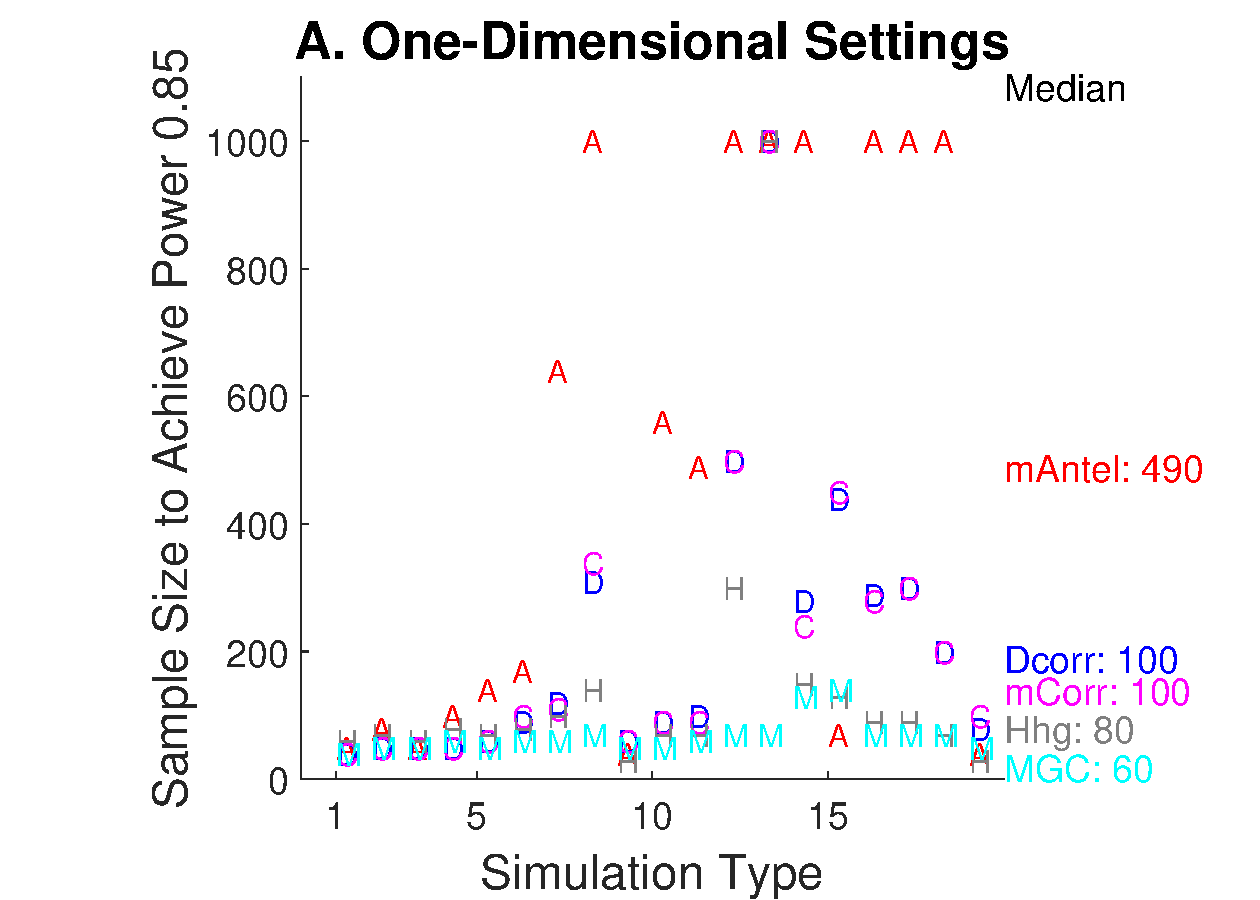
\includegraphics[width=0.9\textwidth,trim={1.5cm 0 0cm 0cm},clip]{../../figs/Fig1DPowerSummarySize}
\end{subfigure}
\centering
\begin{subfigure}[t]{0.45\textwidth}
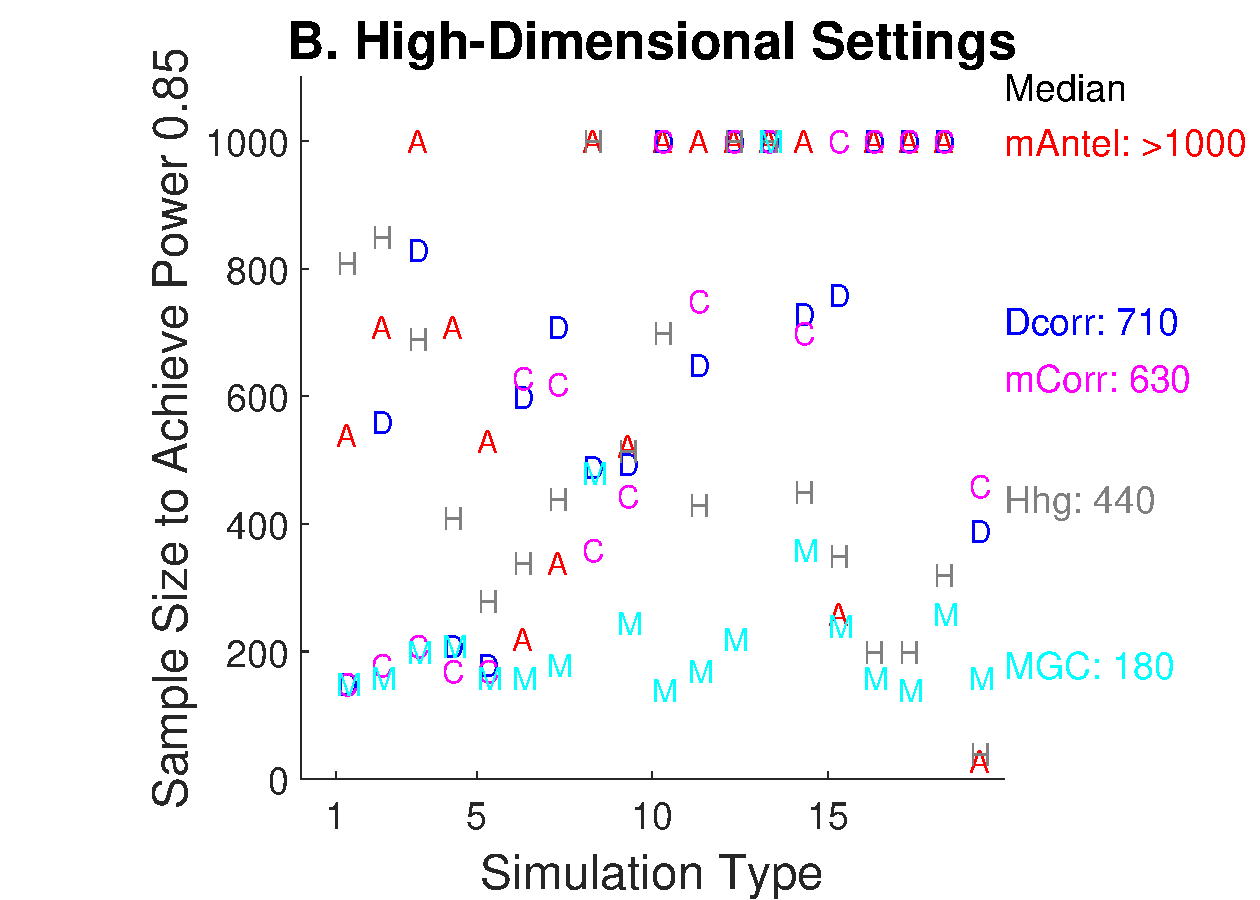
\includegraphics[width=0.9\textwidth,trim={1.5cm 0 0cm 0cm},clip]{../../figs/FigHDPowerSummarySize}
\end{subfigure}
    \caption{Sample size of different methods to achieve a power of $85\%$ at type 1 error level $0.05$, for the $20$ different settings under 1-dimensional (A) and high-dimensional (B) settings.
The x-axis is the simulation type, and y-axis shows the minimal sample size of each method to achieve the required testing power, the smaller the better.
% For panel (A), the dimension is fixed at $1$ for each setting, and the minimal size to achieve the required testing power is estimated. 
%For panel (B), the dimension for each setting is chosen on the basis of the experiments in Supplementary Figure~\ref{f:nDAll}. 
% https://www.ncbi.nlm.nih.gov/pmc/articles/PMC3826013/. 
We bound the sample size to $1000$ in visualization, with the median sample size for each method reported in the far right column. The results indicate that \Mgc~is a superior choice for finite-sample dependency testing, e.g., for the second best method \Hhg, on the median it requires greater than twice the sample size of \Mgc~to achieve the same power.}
		\label{fig:mgcall}
		\end{cframed}
\end{figure}

\clearpage
\end{document}
